\chapter{Probabilistic Models} \label{chap:models}

\section*{}

\section{Introduction}

Probabilistic or statistical models represent explicit assumptions about a problem domain, in the form of a model. This model usually encompasses random variables\footnote{Variable whose value is given by a probability distribution, commonly represented by $\theta$.}, in the form of probability distributions, and the relation and dependence between the variables. \cite{Winn2013}

In the following sections we describe a common way to represent probabilistic models, probabilistic graphical models (PGM) or, simply, graphical models.

\section{Probabilistic Graphical Models}

A PGM is a probabilistic models based on a graph where the nodes represent random variables and the (directed) edges represent a conditional dependence between variables. An example is shown in figure \ref{fig:pgm}.

\begin{figure}[h]
	\begin{center}
		\leavevmode
		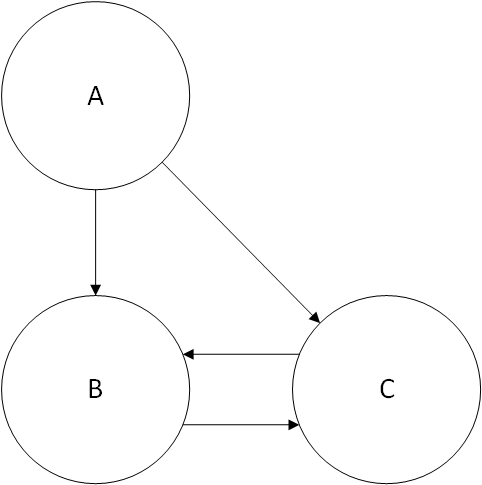
\includegraphics[width=0.36\textwidth]{pgm}
		\caption{Example of a PGM: B and C depend on A, B depends on C and C depends on B. }
		\label{fig:pgm}
	\end{center}
\end{figure}

PGMs and their extensions, where we show some examples of them in the following sections, are exceptionally well suited for reasoning and to reach conclusions based on available information (both domain expert and data), even in the presence of uncertainty. PGMs provide a general framework that allows representation, inference and learning on these models. \cite{koller2009probabilistic}

There is extensive research and available literature in this area. Some notable examples include, but are not limited to, the books \textit{"Probabilistic Graphical Models: Principles and Techniques"} by Daphne Koller and Nir Friedman \cite{koller2009probabilistic} and \textit{"Pattern Recognition and Machine Learning"} (Chapter 8: Graphical Models) by Christopher Bishop \cite{bishop2006pattern}. It is also worth mentioning that there is a MOOC \footnote{Massive Open Online Course} named \textit{"Probabilistic Graphical Models"}, also by Daphne Koller (Stanford), freely available on Coursera \footnote{https://www.coursera.org/course/pgm}.

In the following sections, we describe three important types of graphical models: Bayesian networks, Markov random fields and its extension to hidden Markov models. There are many other graphical models however they were deemed not relevant enough to be included in this literature review.

\section{Bayesian Networks}

\section{Markov Random Fields}

\section{Hidden Markov Models}

\cite{Rabiner1989}

\section{Summary}
